\documentclass[11pt,a4paper]{article}

% === Fonts ===
\usepackage{fourier}  % Utopia-based font with matching math (loads T1 fontenc internally)
\usepackage[utf8]{inputenc}

% === Math ===
\usepackage{amsmath}
\usepackage{amssymb}
\usepackage{mathtools}

% === Layout ===
\usepackage[margin=2cm]{geometry}
\usepackage{parskip}

% === Colors and boxes ===
\usepackage[dvipsnames]{xcolor}
\usepackage[most]{tcolorbox}

% === Hyperlinks ===
\usepackage{hyperref}
\hypersetup{colorlinks=true, linkcolor=blue, urlcolor=blue}

% === Allow line breaks in equations ===
\allowdisplaybreaks

% === Custom commands ===
\newcommand{\R}{\mathbb{R}}
\newcommand{\bx}{\mathbf{x}}
\newcommand{\bu}{\mathbf{u}}
\newcommand{\bv}{\mathbf{v}}
\newcommand{\bp}{\mathbf{p}}
\newcommand{\be}{\mathbf{e}}
\newcommand{\MLP}{\operatorname{MLP}}
\newcommand{\attn}{\operatorname{Attn}}
\newcommand{\Logit}{\operatorname{Logit}}
\newcommand{\FVE}{\operatorname{FVE}}
\newcommand{\ReLU}{\operatorname{ReLU}}
\DeclareMathOperator*{\argmax}{arg\,max}

\title{Fourier Multiplication Circuit\\[6pt]
\large Discovered in a 1-Layer Transformer Trained on $(a + b) \bmod 113$}
\author{Auto-generated by Grokking Circuit Discovery Tool}
\date{\today}

\begin{document}
\maketitle

\begin{tcolorbox}[colback=blue!5!white, colframe=blue!75!black, title=Circuit Summary]
  \textbf{Task:} $(a + b) \bmod 113$ \hfill
  \textbf{FVE:} 0.9395 \hfill
  \textbf{Formula Accuracy:} 100.00\%

  \textbf{Key frequencies:} $\mathcal{K} = \{16, 31, 43, 52, 53\}$
  \quad (5 frequencies)

  \textbf{Neurons assigned:} 1/512
  \quad ($k=16$: 1, $k=31$: 0, $k=43$: 0, $k=52$: 0, $k=53$: 0)
\end{tcolorbox}

\begin{tcolorbox}[colback=green!5!white, colframe=green!75!black, title=The Core Equation]
  \begin{equation}
    \boxed{
      \Logit(c \mid a, b) =
      \sum_{k \in \mathcal{K}}
      \underbrace{\alpha_k}_{\substack{\text{learned} \\ \text{amplitude}}}
      \cdot \underbrace{\cos\!\left(\frac{2\pi k (a + b - c)}{113}\right)}_{\substack{\text{max at } c = (a+b) \bmod 113 \\ \text{(constructive interference)}}}
    }
  \end{equation}
\end{tcolorbox}

\begin{tcolorbox}[colback=orange!5!white, colframe=orange!75!black, title=Data Flow Pipeline]
  \begin{gather*}
    \underbrace{a, b}_{\text{inputs}}
    \xrightarrow{\; W_E \;}
    \underbrace{\cos(\omega_k t),\; \sin(\omega_k t)}_{\text{Fourier embedding}}
    \xrightarrow{\; \attn \;}
    \underbrace{\text{degree-2 products}}_{\substack{\text{attn wt.} \times \text{OV}}} \\[8pt]
    \xrightarrow{\; \MLP \;}
    \underbrace{\cos(\omega_k(a{+}b)),\; \sin(\omega_k(a{+}b))}_{\text{trig addition identities}}
    \xrightarrow{\; W_U \;}
    \underbrace{\cos(\omega_k(a{+}b{-}c))}_{\text{logits}}
  \end{gather*}
\end{tcolorbox}

\tableofcontents
\newpage

\section{Variable Definitions}

Every symbol used in this document is defined below. Refer back to this table whenever a variable is unclear.

\begin{longtable}
\hline
\textbf{Symbol} & \textbf{Name / Meaning} & \textbf{Shape / Value} \\ \hline
\endhead
\multicolumn{3}{|c|}{\textit{Scalar Constants}} \\ \hline
  $P$ & Prime modulus. The model computes $(a+b) \bmod P$. & $113$ \\ \hline
  $d_{\text{model}}$ & Dimension of the residual stream (embedding size). & $128$ \\ \hline
  $d_{\text{mlp}}$ & Number of neurons in the MLP hidden layer. & $512$ \\ \hline
  $d_{\text{head}}$ & Dimension of each attention head's Q/K/V vectors. Equal to $d_{\text{model}} / n_{\text{heads}}$. & $32$ \\ \hline
  $n_{\text{heads}}$ & Number of attention heads. & $4$ \\ \hline
  $k$ & A frequency index. Ranges over $\mathcal{K}$. & Integer in $\{1, \ldots, 56\}$ \\ \hline
  $\omega_k$ & Angular frequency for index $k$. Defined as $\omega_k = \frac{2\pi k}{P}$. & $\frac{2\pi k}{113}$ radians \\ \hline
  $\mathcal{K}$ & Set of key frequencies discovered via Fourier analysis of $W_E$ and $W_L$. & $\{16, 31, 43, 52, 53\}$ \\ \hline
\multicolumn{3}{|c|}{\textit{Tokens and Positions}} \\ \hline
  $a$ & The first input token (an integer). Sits at position 0 in the sequence. & $a \in \{0, \ldots, 112\}$ \\ \hline
  $b$ & The second input token (an integer). Sits at position 1 in the sequence. & $b \in \{0, \ldots, 112\}$ \\ \hline
  $=$ & The equals-sign token. A special fixed token at position 2. The model reads its output from this position. & Token index $= P = 113$ \\ \hline
  $c$ & A candidate output class. The model produces a logit for each $c$. & $c \in \{0, \ldots, 112\}$ \\ \hline
  $c^*$ & The correct answer: $c^* = (a + b) \bmod P$. & $(a+b) \bmod 113$ \\ \hline
  $\mathbf{e}_a$ & One-hot vector for token $a$. Has a 1 in position $a$ and 0 elsewhere. This is the raw input to the embedding matrix. & $\in \mathbb{R}^{114}$ \\ \hline
  $\mathbf{e}_b$ & One-hot vector for token $b$. & $\in \mathbb{R}^{114}$ \\ \hline
  position 0 & The first slot in the 3-token input sequence ``$a\ b\ =$''. Token $a$ lives here. & --- \\ \hline
  position 1 & The second slot. Token $b$ lives here. & --- \\ \hline
  position 2 & The third slot. The ``$=$'' token lives here. All output logits are read from this position. & --- \\ \hline
\multicolumn{3}{|c|}{\textit{Weight Matrices}} \\ \hline
  $W_E$ & Token embedding matrix. Maps one-hot token vectors to $d_{\text{model}}$-dimensional vectors. Row $a$ of $W_E$ is the embedding of token $a$. & $\in \mathbb{R}^{114 \times 128}$ \\ \hline
  $\mathbf{p}_i$ & Positional embedding for position $i \in \{0, 1, 2\}$. Added to the token embedding to form the initial residual stream. & $\in \mathbb{R}^{128}$ \\ \hline
  $W_Q^{(j)}$ & Query weight matrix for attention head $j$. Projects the residual stream at the query position into query space. & $\in \mathbb{R}^{128 \times 128}$ \\ \hline
  $W_K^{(j)}$ & Key weight matrix for attention head $j$. Projects the residual stream at key positions into key space. & $\in \mathbb{R}^{128 \times 128}$ \\ \hline
  $W_V^{(j)}$ & Value weight matrix for attention head $j$. Projects the residual stream at value positions into value space. & $\in \mathbb{R}^{128 \times 128}$ \\ \hline
  $W_O^{(j)}$ & Output projection matrix for attention head $j$. Projects the attention output back to the residual stream. & $\in \mathbb{R}^{128 \times 128}$ \\ \hline
  $W_{\text{in}}$ & MLP input weight matrix. Projects from residual stream to MLP hidden layer. & $\in \mathbb{R}^{512 \times 128}$ \\ \hline
  $b_{\text{in}}$ & MLP input bias vector. & $\in \mathbb{R}^{512}$ \\ \hline
  $W_{\text{out}}$ & MLP output weight matrix. Projects from MLP hidden layer back to residual stream. & $\in \mathbb{R}^{128 \times 512}$ \\ \hline
  $W_U$ & Unembedding matrix. Maps final residual stream to output logits (one per class $c$). & $\in \mathbb{R}^{113 \times 128}$ \\ \hline
  $W_L$ & Neuron-logit map. Defined as $W_L = W_{\text{out}}^\top \cdot W_U^\top$. Maps MLP neuron activations directly to output logits. This is the key matrix for Fourier analysis. & $\in \mathbb{R}^{512 \times 113}$ \\ \hline
\multicolumn{3}{|c|}{\textit{Intermediate Activations}} \\ \hline
  $\mathbf{x}^{(0)}_a$ & Initial residual stream at position 0 (where token $a$ sits). Equals $W_E \cdot \mathbf{e}_a + \mathbf{p}_0$. & $\in \mathbb{R}^{128}$ \\ \hline
  $\mathbf{x}^{(0)}_b$ & Initial residual stream at position 1 (where token $b$ sits). Equals $W_E \cdot \mathbf{e}_b + \mathbf{p}_1$. & $\in \mathbb{R}^{128}$ \\ \hline
  $\mathbf{x}^{(0)}_=$ & Initial residual stream at position 2 (the ``$=$'' token). This is constant (independent of $a, b$) since the token and position are fixed. & $\in \mathbb{R}^{128}$ \\ \hline
  $\mathbf{x}^{(1)}$ & Residual stream at position 2 after the attention layer. Equals $\mathbf{x}^{(0)}_= + \sum_j \text{attn\_out}^{(j)}$. & $\in \mathbb{R}^{128}$ \\ \hline
  $A^{(j)}_0$ & Attention weight from head $j$ at position 2 (``$=$'') attending to position 0 (token $a$). A scalar between 0 and 1. Note: $A^{(j)}_1 = 1 - A^{(j)}_0$. & Scalar $\in [0, 1]$ \\ \hline
  $A^{(j)}_1$ & Attention weight from head $j$ at position 2 attending to position 1 (token $b$). Equals $1 - A^{(j)}_0$. & Scalar $\in [0, 1]$ \\ \hline
  $\text{MLP}[n]$ & Activation of MLP neuron $n$ (after ReLU). Equals $\max(0,\; W_{\text{in}}[n,:] \cdot \mathbf{x}^{(1)} + b_{\text{in}}[n])$. & Scalar $\geq 0$; $n \in \{0, \ldots, 511\}$ \\ \hline
  $\text{Logit}(c)$ & Output logit for class $c$. The model predicts $\hat{c} = \arg\max_c \text{Logit}(c)$. & Scalar \\ \hline
\multicolumn{3}{|c|}{\textit{Fourier Analysis Variables}} \\ \hline
  $\alpha_k$ & Amplitude coefficient for frequency $k$ in the logit formula. Fitted via OLS: $\text{Logit}(c) \approx \sum_k \alpha_k \cos(\omega_k(a+b-c))$. Larger $\alpha_k$ means frequency $k$ contributes more to the final prediction. & $\alpha_{16}$, $\alpha_{31}$, $\alpha_{43}$, $\alpha_{52}$, $\alpha_{53}$ \\ \hline
  $\beta_k$ & Amplitude of the sine component in the embedding. Measures how strongly $W_E$ encodes $\sin(\omega_k \cdot t)$ for token $t$. Analogous to $\alpha_k$ but for the sine direction. & Fitted from $W_E$ Fourier decomposition \\ \hline
  $\mathbf{u}_k$ & Direction in neuron space ($\mathbb{R}^{512}$) along which the MLP encodes $\cos(\omega_k(a+b))$. Extracted from the Fourier decomposition of $W_L$: the column of $W_L$ in the Fourier basis corresponding to $\cos(\omega_k c)$. & $\in \mathbb{R}^{512}$ \\ \hline
  $\mathbf{v}_k$ & Direction in neuron space along which the MLP encodes $\sin(\omega_k(a+b))$. The column of $W_L$ in the Fourier basis corresponding to $\sin(\omega_k c)$. & $\in \mathbb{R}^{512}$ \\ \hline
  $\mathbf{u}_k^{(\cos)}$ & Direction in residual stream ($\mathbb{R}^{128}$) along which the embedding encodes the cosine component at frequency $k$. Extracted from the Fourier decomposition of $W_E$. & $\in \mathbb{R}^{128}$ \\ \hline
  $\mathbf{u}_k^{(\sin)}$ & Direction in residual stream along which the embedding encodes the sine component at frequency $k$. & $\in \mathbb{R}^{128}$ \\ \hline
  $\gamma_j$ & Modulation amplitude of attention head $j$. Measures how much head $j$'s attention pattern deviates from uniform (0.5). Comes from the linear approximation to the sigmoid of the attention score difference. & Scalar (typically $|\gamma_j| \approx 0.25$) \\ \hline
  $C^{(j)}$ & Attention score lookup vector for head $j$. Defined as $C^{(j)} = W_E^\top W_K^{(j)\top} W_Q^{(j)} \mathbf{x}^{(0)}_=$. Entry $C^{(j)}[a]$ gives the attention score contribution from token $a$. & $\in \mathbb{R}^{113}$ \\ \hline
  $0.5$ (baseline) & When softmax is applied over exactly 2 elements, the result is $\sigma(\Delta) = \frac{1}{1 + e^{-\Delta}}$. At $\Delta = 0$ (no preference), this equals $0.5$. So 0.5 is the ``no information'' baseline for attention over 2 positions. & Constant \\ \hline
\end{longtable}

\textbf{Note on the ``$=$'' token:} The input to the model is the 3-token sequence ``$a\;\; b\;\; =$''. The ``$=$'' is a literal token (with its own embedding) that serves as the query position from which the model reads its output. It is \emph{not} the mathematical equals sign. Its embedding $\mathbf{x}^{(0)}_=$ is constant across all inputs.

\section{Circuit Architecture (TikZ Diagram)}

\begin{figure}[htbp]
\centering
\resizebox{\textwidth}{!}{%
\begin{tikzpicture}[
    node distance=2.0cm and 3.0cm,
    block/.style={rectangle, draw, rounded corners, minimum width=3.2cm,
        minimum height=1.1cm, align=center, font=\small},
    data/.style={rectangle, draw, dashed, rounded corners, minimum width=3cm,
        minimum height=0.8cm, align=center, font=\footnotesize, fill=yellow!10},
    arrow/.style={->, >=stealth, thick},
    lbl/.style={font=\scriptsize, align=center},
    ]

    % === INPUT LAYER ===
    \node[block, fill=orange!20] (input_a) {Token $a$\\(position 0)};
    \node[block, fill=orange!20, right=3cm of input_a] (input_b) {Token $b$\\(position 1)};
    \node[block, fill=orange!20, right=3cm of input_b] (input_eq) {Token ``$=$''\\(position 2)};

    % === EMBEDDING LAYER ===
    \draw[arrow] (unembed) -- node[right, lbl] {logits $\in \mathbb{R}^{113}$} (output);

    % === FREQUENCY ANNOTATION ===
    \node[draw, rounded corners, fill=gray!10, font=\footnotesize,
        text width=4.5cm, align=center, right=2.5cm of embed_eq] (freq_box) {
        \textbf{Key Frequencies}\\$\mathcal{K} = \{16, 31, 43, 52, 53\}$\\[3pt]
        $\omega_k = \frac{2\pi k}{113}$};

\end{tikzpicture}
}
\caption{Data flow pipeline of the Fourier multiplication circuit. 
Tokens $a$ and $b$ are embedded into Fourier components, attention moves them to the output position, 
the MLP computes trigonometric addition identities, and the unembedding reads off logits via constructive interference.}
\label{fig:pipeline}
\end{figure}

% =============================================================
% FOURIER MULTIPLICATION CIRCUIT — FULL DERIVATION
% P = 113, key frequencies k ∈ {16, 31, 43, 52, 53}
% =============================================================
\section{Discovered Circuit: Fourier Multiplication Algorithm}

The model computes $(a + b) \bmod 113$ using a 1-layer transformer with $d_{\text{model}} = 128$, $n_{\text{heads}} = 4$, $d_{\text{mlp}} = 512$. It uses 5 key frequencies $k \in \mathcal{K} = \{16, 31, 43, 52, 53\}$ with angular frequencies $\omega_k = \frac{2\pi k}{113}$.

Each equation below is presented at three levels:
\begin{enumerate}
  \item \textbf{Abstract:} What the step does in plain English.
  \item \textbf{Symbolic:} Full equations with every variable underbraced by name.
  \item \textbf{Concrete:} Actual numerical values from the trained model (example: $a = 7$, $b = 13$, $c^* = 20$).
\end{enumerate}

\subsection{Step 1: Embedding (Token $\to$ Fourier Components)}

\subsubsection*{Abstract}
Each input token $t$ (an integer $0$ to $112$) is converted into a $d_{\text{model}}$-dimensional vector by looking up row $t$ of the embedding matrix $W_E$ and adding a positional embedding. The key property of $W_E$ (learned during training) is that its rows, when projected onto the Fourier basis, are dominated by sinusoidal components at the key frequencies $\mathcal{K}$. This means the embedding effectively encodes each token as $\cos(\omega_k \cdot t)$ and $\sin(\omega_k \cdot t)$ for each key frequency $k$.

\subsubsection*{Symbolic}
\begin{align}
    \underbrace{\mathbf{x}^{(0)}_a}_{\substack{\text{initial residual stream} \\ \text{at position 0} \\ \in \mathbb{R}^{128}}} &= \underbrace{W_E \cdot \mathbf{e}_a}_{\substack{\text{row } a \text{ of the} \\ \text{embedding matrix} \\ \in \mathbb{R}^{128}}} + \underbrace{\mathbf{p}_0}_{\substack{\text{positional embedding} \\ \text{for position 0} \\ \in \mathbb{R}^{128}}} \\
    &\approx \sum_{k \in \mathcal{K}} \bigg[ \underbrace{\alpha_k}_{\substack{\text{cosine amplitude} \\ \text{(from Fourier} \\ \text{decomp of } W_E\text{)}}} \underbrace{\cos\!\left(\frac{2\pi k \cdot a}{113}\right)}_{\substack{\text{cosine evaluated} \\ \text{at token } a}}\cdot \underbrace{\mathbf{u}_k^{(\cos)}}_{\substack{\text{direction in } \mathbb{R}^{128} \\ \text{for } \cos \text{ at freq } k}} + \underbrace{\beta_k}_{\substack{\text{sine amplitude} \\ \text{(from Fourier} \\ \text{decomp of } W_E\text{)}}} \underbrace{\sin\!\left(\frac{2\pi k \cdot a}{113}\right)}_{\substack{\text{sine evaluated} \\ \text{at token } a}}\cdot \underbrace{\mathbf{u}_k^{(\sin)}}_{\substack{\text{direction in } \mathbb{R}^{128} \\ \text{for } \sin \text{ at freq } k}} \bigg]
\end{align}

\subsubsection*{Concrete (for $a = 7$, $b = 13$)}

Evaluating the Fourier components for each key frequency:
\begin{center}
\begin{tabular}{|c|c|c|c|c|}
\hline
$k$ & $\omega_k$ & $\cos(\omega_k \cdot 7)$ & $\sin(\omega_k \cdot 7)$ & $\cos(\omega_k \cdot 13)$ \\ \hline
  $16$ & $\frac{2\pi \cdot 16}{113} = 0.8897$ & $0.9985$ & $-0.0556$ & $0.5396$ \\ \hline
  $31$ & $\frac{2\pi \cdot 31}{113} = 1.7237$ & $0.8774$ & $-0.4798$ & $-0.9143$ \\ \hline
  $43$ & $\frac{2\pi \cdot 43}{113} = 2.3909$ & $-0.5160$ & $-0.8566$ & $0.9449$ \\ \hline
  $52$ & $\frac{2\pi \cdot 52}{113} = 2.8914$ & $0.1797$ & $0.9837$ & $0.9938$ \\ \hline
  $53$ & $\frac{2\pi \cdot 53}{113} = 2.9470$ & $-0.2070$ & $0.9783$ & $0.8187$ \\ \hline
\end{tabular}
\end{center}

\subsection{Step 2: Attention (Move Fourier Info to Output Position)}

\subsubsection*{Abstract}
The attention layer's job is to move information from positions 0 and 1 (where tokens $a$ and $b$ live) to position 2 (the ``$=$'' token, from which the model reads its output). Each of the 4 attention heads computes a query from the ``$=$'' position and keys from positions 0 and 1. Since softmax over exactly 2 elements is a sigmoid, each head produces an attention weight $A^{(j)}_0 \in [0, 1]$ (with $A^{(j)}_1 = 1 - A^{(j)}_0$). The ``uniform baseline'' of $0.5$ means the head attends equally to both positions (no preference). Deviations from $0.5$ encode periodic information about the inputs.

\subsubsection*{Symbolic}
\begin{align}
    \underbrace{\text{score}^{(j)}_{= \to a}}_{\substack{\text{attention score from} \\ \text{``='' to position 0}}} &= \frac{\overbrace{\mathbf{x}^{(0)}_= \cdot W_Q^{(j)}}^{\substack{\text{query vector} \\ \text{(from ``='' at pos 2)} \\ \in \mathbb{R}^{32}}}\;\cdot\; \overbrace{\left(W_K^{(j)}\right)^\top \!\cdot \mathbf{x}^{(0)}_a}^{\substack{\text{key vector} \\ \text{(from token } a \text{ at pos 0)} \\ \in \mathbb{R}^{32}}}}{\underbrace{\sqrt{d_{\text{head}}}}_{\substack{\text{scaling factor} \\ = \sqrt{32} = 5.66}}} \\
    \underbrace{A^{(j)}_0}_{\substack{\text{attention weight} \\ \text{from ``='' to } a \\ \in [0, 1]}} &= \underbrace{\sigma\!\left(\text{score}^{(j)}_{= \to a} - \text{score}^{(j)}_{= \to b}\right)}_{\substack{\text{softmax over 2 elements} \\ = \text{sigmoid of score difference} \\ \sigma(x) = \frac{1}{1 + e^{-x}}}} \\
    &\approx \underbrace{0.5}_{\substack{\text{uniform baseline:} \\ \sigma(0) = 0.5 \\ \text{(no preference)}}} + \underbrace{\gamma_j}_{\substack{\text{modulation} \\ \text{amplitude} \\ \text{(from linear} \\ \text{approx of } \sigma\text{)}}} \Big(\underbrace{\cos\!\left(\omega_{k_j} \cdot a\right)}_{\substack{\text{periodic score} \\ \text{for token } a}} - \underbrace{\cos\!\left(\omega_{k_j} \cdot b\right)}_{\substack{\text{periodic score} \\ \text{for token } b}}\Big) \\
    \underbrace{\text{attn\_out}^{(j)}}_{\substack{\text{attention output} \\ \text{of head } j \\ \in \mathbb{R}^{128}}} &= \underbrace{A^{(j)}_0}_{\text{weight to } a} \cdot \overbrace{W_O^{(j)} W_V^{(j)} \mathbf{x}^{(0)}_a}^{\substack{\text{OV circuit on } a \\ \text{(value} \to \text{output projection)}}} + \underbrace{(1 - A^{(j)}_0)}_{\text{weight to } b} \cdot \overbrace{W_O^{(j)} W_V^{(j)} \mathbf{x}^{(0)}_b}^{\substack{\text{OV circuit on } b}}
\end{align}

\subsubsection*{Concrete (for $a = 7$, $b = 13$)}

Actual attention weights extracted from the model:
\begin{center}
\begin{tabular}{|c|c|c|c|}
\hline
Head $j$ & $A^{(j)}_0$ (to $a$) & $A^{(j)}_1$ (to $b$) & Deviation from 0.5 \\ \hline
  0 & $0.5000$ & $0.5000$ & $+0.0000$ \\ \hline
  1 & $0.5000$ & $0.5000$ & $+0.0000$ \\ \hline
  2 & $0.5000$ & $0.5000$ & $+0.0000$ \\ \hline
  3 & $0.5000$ & $0.5000$ & $+0.0000$ \\ \hline
\end{tabular}
\end{center}

\textbf{Interpretation:} Deviations from $0.5$ encode periodic information. A head with $A^{(j)}_0 > 0.5$ attends more to token $a$; this modulation is periodic in $a$ and $b$ at the head's tuned frequency $k_j$.

\subsection{Step 3: MLP (Compute Trig Identities)}

\subsubsection*{Abstract}
The residual stream after attention contains degree-2 products of sines and cosines (because attention weight $\times$ OV output = linear $\times$ linear = quadratic). The MLP's 512 neurons, via ReLU activation, collectively implement the trigonometric addition identities that convert these products into $\cos(\omega_k(a+b))$ and $\sin(\omega_k(a+b))$. This is the core computational step.

\subsubsection*{Symbolic}
\begin{align}
    \underbrace{\mathbf{x}^{(1)}}_{\substack{\text{residual stream} \\ \text{after attention} \\ \in \mathbb{R}^{128}}} &= \underbrace{\mathbf{x}^{(0)}_=}_{\substack{\text{skip connection} \\ \text{(``='' token embedding} \\ \text{+ pos embed)}}} + \sum_{j=0}^{3} \underbrace{\text{attn\_out}^{(j)}}_{\substack{\text{head } j \text{ output} \\ \text{(degree-2 trig)}}} \\
    \underbrace{\text{pre}_n}_{\substack{\text{pre-activation} \\ \text{of neuron } n \\ \text{(scalar)}}} &= \underbrace{W_{\text{in}}[n, :]}_{\substack{\text{row } n \text{ of MLP} \\ \text{input matrix} \\ \in \mathbb{R}^{128}}} \cdot \underbrace{\mathbf{x}^{(1)}}_{\substack{\text{residual stream} \\ \text{(input to MLP)}}} + \underbrace{b_{\text{in}}[n]}_{\substack{\text{bias for} \\ \text{neuron } n}} \\
    \underbrace{\text{MLP}[n]}_{\substack{\text{activation of} \\ \text{neuron } n \\ \text{(after ReLU)} \\ \geq 0}} &= \underbrace{\max(0,\; \text{pre}_n)}_{\substack{\text{ReLU: zero out} \\ \text{negative values} \\ \text{(creates piecewise-linear} \\ \text{approx of trig products)}}}
\end{align}

\textbf{The core computation:} For each key frequency $k$, the MLP neurons collectively compute the addition formula:
\begin{align}
    \underbrace{\mathbf{u}_k^\top \cdot \text{MLP}(a,b)}_{\substack{\text{dot product of all } 512 \text{ neuron} \\ \text{activations with direction } \mathbf{u}_k \\ \text{(extracted from } W_L = W_{\text{out}}^\top W_U^\top \text{)}}} &\approx \underbrace{\alpha_k}_{\substack{\text{amplitude} \\ \text{coefficient}}} \underbrace{\cos\!\left(\omega_k(a+b)\right)}_{\substack{\text{cosine of the SUM} \\ \text{(this is the target)}}} \\
    &= \underbrace{\alpha_k \cos(\omega_k a) \cos(\omega_k b)}_{\substack{\text{from neurons computing} \\ \text{cos} \times \text{cos products}}} - \underbrace{\alpha_k \sin(\omega_k a) \sin(\omega_k b)}_{\substack{\text{from neurons computing} \\ \text{sin} \times \text{sin products}}}
\end{align}

\subsubsection*{Concrete (for $a = 7$, $b = 13$)}

Of the 512 neurons, \textbf{?} are active (positive after ReLU) for this input.

Projecting the MLP activations onto the Fourier directions $\mathbf{u}_k$ and $\mathbf{v}_k$:
\begin{center}
\begin{tabular}{|c|c|c|c|c|}
\hline
$k$ & $\mathbf{u}_k^\top \cdot \text{MLP}$ & $\alpha_k \cos(\omega_k(a+b))$ & $\cos(\omega_k \cdot 20)$ & $\alpha_k$ \\ \hline
  $16$ & ? & ? & $0.4920$ & ? \\ \hline
  $31$ & ? & ? & $-0.9965$ & ? \\ \hline
  $43$ & ? & ? & $-0.7680$ & ? \\ \hline
  $52$ & ? & ? & $0.2878$ & ? \\ \hline
  $53$ & ? & ? & $-0.7312$ & ? \\ \hline
\end{tabular}
\end{center}

\textbf{Verifying the trig identity for the first key frequency $k = 16$:}

\begin{align*}
    &\underbrace{\cos\!\left(\frac{2\pi \cdot 16 \cdot 7}{113}\right)}_{= 0.9985} \cdot \underbrace{\cos\!\left(\frac{2\pi \cdot 16 \cdot 13}{113}\right)}_{= 0.5396} - \underbrace{\sin\!\left(\frac{2\pi \cdot 16 \cdot 7}{113}\right)}_{= -0.0556} \cdot \underbrace{\sin\!\left(\frac{2\pi \cdot 16 \cdot 13}{113}\right)}_{= -0.8419} \\
    &= (0.9985)(0.5396) - (-0.0556)(-0.8419) \\
    &= 0.5387 - 0.0468 \\
    &= 0.4920 \\
    &= \underbrace{\cos\!\left(\frac{2\pi \cdot 16 \cdot (7+13)}{113}\right)}_{= \cos\!\left(\frac{2\pi \cdot 16 \cdot 20}{113}\right) = 0.4920} \quad \checkmark
\end{align*}

\subsection{Step 4: Unembedding (Fourier $\to$ Logits)}

\subsubsection*{Abstract}
The neuron-logit map $W_L = W_{\text{out}}^\top \cdot W_U^\top$ converts the MLP neuron activations directly into output logits. Its key property (discovered via Fourier analysis) is that it is approximately rank 10: it decomposes into 5 pairs of directions, one pair per key frequency. Each pair reads off $\cos(\omega_k(a+b))$ and $\sin(\omega_k(a+b))$ from the MLP activations and multiplies them by $\cos(\omega_k c)$ and $\sin(\omega_k c)$ respectively. By the cosine subtraction identity, this produces $\cos(\omega_k(a+b-c))$.

\subsubsection*{Symbolic}
\begin{align}
    \underbrace{W_L}_{\substack{\text{neuron-logit map} \\ \in \mathbb{R}^{512 \times 113} \\ = W_{\text{out}}^\top W_U^\top}} &\approx \sum_{k \in \mathcal{K}} \bigg[ \underbrace{\cos(\omega_k c)}_{\substack{\text{vector in } \mathbb{R}^{113} \\ \text{whose } c\text{-th entry} \\ \text{is } \cos(\omega_k c)}} \cdot \underbrace{\mathbf{u}_k^\top}_{\substack{\text{row vector in } \mathbb{R}^{512} \\ \text{reads } \cos(\omega_k(a+b)) \\ \text{from MLP activations}}} + \underbrace{\sin(\omega_k c)}_{\substack{\text{vector in } \mathbb{R}^{113} \\ \text{whose } c\text{-th entry} \\ \text{is } \sin(\omega_k c)}} \cdot \underbrace{\mathbf{v}_k^\top}_{\substack{\text{row vector in } \mathbb{R}^{512} \\ \text{reads } \sin(\omega_k(a+b)) \\ \text{from MLP activations}}} \bigg] \\
    \underbrace{\text{Logit}(c \mid a, b)}_{\substack{\text{output logit} \\ \text{for class } c}} &= \underbrace{W_L^\top \cdot \text{MLP}(a,b)}_{\substack{\text{neuron-logit map} \\ \text{applied to MLP output}}} \\
    &\approx \sum_{k \in \mathcal{K}} \bigg[ \underbrace{\cos(\omega_k c)}_{\substack{\text{from } W_L \\ \text{(unembed)}}} \cdot \underbrace{\mathbf{u}_k^\top \text{MLP}(a,b)}_{\substack{\approx \alpha_k \cos(\omega_k(a+b)) \\ \text{(MLP computed this)}}} + \underbrace{\sin(\omega_k c)}_{\substack{\text{from } W_L \\ \text{(unembed)}}} \cdot \underbrace{\mathbf{v}_k^\top \text{MLP}(a,b)}_{\substack{\approx \alpha_k \sin(\omega_k(a+b)) \\ \text{(MLP computed this)}}} \bigg] \\
    &= \sum_{k \in \mathcal{K}} \underbrace{\alpha_k}_{\substack{\text{amplitude} \\ \text{coefficient}}} \underbrace{\Big[\cos(\omega_k c)\cos(\omega_k(a+b)) + \sin(\omega_k c)\sin(\omega_k(a+b))\Big]}_{\substack{\text{cosine subtraction identity:} \\ \cos(X)\cos(Y) + \sin(X)\sin(Y) = \cos(X - Y)}} \\
    &= \boxed{\sum_{k \in \mathcal{K}} \underbrace{\alpha_k \cos\!\left(\omega_k(a + b - c)\right)}_{\substack{\text{peaks when } c \equiv a+b \pmod{113} \\\text{since } \cos(0) = 1 \text{ is the maximum}}}}
\end{align}

\subsubsection*{Concrete (for $a = 7$, $b = 13$, $c^* = 20$)}

\begin{itemize}
\end{itemize}

Evaluating the formula at $c^* = 20$:
\begin{align*}
    \text{Logit}(20) &= \sum_{k \in \mathcal{K}} \alpha_k \cos\!\left(\omega_k \cdot \underbrace{(7 + 13 - 20)}_{= 0 = 0}\right) \\
\end{align*}

\subsection{Step 5: Prediction via Constructive Interference}

\subsubsection*{Abstract}
The model predicts the class $c$ with the highest logit. Because the logit formula is a sum of cosines $\sum_k \alpha_k \cos(\omega_k(a+b-c))$, and $\cos(0) = 1$ is the maximum of cosine, ALL cosines simultaneously achieve their maximum when $c \equiv a + b \pmod{113}$. This is \textbf{constructive interference}: all 5 cosine waves peak at the same point. For any other $c$, the cosines at different frequencies point in different directions and partially cancel (\textbf{destructive interference}), giving a smaller logit.

\subsubsection*{Symbolic}
\begin{align}
    \underbrace{\hat{c}}_{\substack{\text{model's} \\ \text{prediction}}} &= \underbrace{\arg\max_{c \in \{0,\ldots,112\}}}_{\text{select class with highest logit}} \overbrace{\sum_{k \in \mathcal{K}} \underbrace{\alpha_k}_{\text{amplitude}} \cos\!\left(\frac{2\pi k (a + b - c)}{113}\right)}^{\text{sum of 5 cosines at key frequencies}} \\
    &= \underbrace{(a + b) \bmod 113}_{\substack{\text{constructive interference:} \\\text{all } 5 \text{ cosines} = 1 \text{ when } c = (a+b) \bmod 113 \\\text{destructive interference for all other } c}}
\end{align}

\subsubsection*{Concrete}
For $a = 7$, $b = 13$: the correct answer is $c^* = (7 + 13) \bmod 113 = 20$.

\begin{itemize}
  \item At $c = c^* = 20$: $a + b - c = 7 + 13 - 20 = 0$ $\equiv 0 \pmod{113}$, so $\cos(\omega_k \cdot 0) = 1$ for ALL $k$.
  \item At $c = 21$ (wrong): $a + b - c \equiv 112 \pmod{113}$, so cosines at different frequencies give different values $\Rightarrow$ partial cancellation.
\end{itemize}

\subsection{Why Multiple Frequencies? (Constructive Interference)}

\subsubsection*{Abstract}
A single cosine $\cos(\omega_k x)$ has period $113$ and achieves its maximum at $x = 0$, but it also comes close to 1 at other values of $x$ (e.g., for $k = 14$: $\cos(\omega_{14} \cdot 8) = 0.998$). A single frequency cannot reliably distinguish $x = 0$ from these near-maxima. By summing cosines at 5 different frequencies, the model constructs a function with a \emph{unique, sharp} maximum at $x = 0 \bmod 113$, because the near-maxima of different frequencies occur at different values of $x$ and thus cancel out.

\subsubsection*{Symbolic}
\begin{align}
    f(x) &= \sum_{k \in \mathcal{K}} \underbrace{\cos\!\left(\frac{2\pi k \cdot x}{113}\right)}_{\text{each has max at } x = 0} \\
    f(0) &= \underbrace{5}_{\text{all } 5 \text{ cosines} = 1} \quad \gg \quad \underbrace{f(x \neq 0)}_{\substack{\text{destructive interference:} \\ \text{cosines at different} \\ \text{frequencies cancel}}}
\end{align}

\subsubsection*{Concrete}
Evaluating $f(x)$ at a few values:
\begin{center}
\begin{tabular}{|c|c|c|}
\hline
$x$ & $f(x) = \sum_k \cos(\omega_k x)$ & Interpretation \\ \hline
  $0$ & $5.0$ & \textbf{Maximum} (all cosines $= 1$) \\ \hline
  $1$ & $-2.2039$ & Partial cancellation \\ \hline
  $2$ & $0.7114$ & Near zero (cancellation) \\ \hline
  $5$ & $-1.0116$ & Partial cancellation \\ \hline
  $56$ & $-0.0873$ & Near zero (cancellation) \\ \hline
\end{tabular}
\end{center}

The ratio $\frac{f(0)}{\max_{x \neq 0} f(x)}$ determines how reliably the model can distinguish the correct answer from all others. With 5 frequencies, this ratio is large enough for the softmax to assign $> 99.99\%$ probability to the correct class.

\subsection{Complete Worked Example: $a=7$, $b=13$}

We now trace the \textbf{entire computation by hand} for the input $(a, b) = (7, 13)$, showing every intermediate value.

\subsubsection*{Step 1: Compute Fourier Components}
\begin{center}
\begin{tabular}{|c|c|c|c|c|c|}
\hline
$k$ & $\omega_k = \frac{2\pi k}{113}$ & $\cos(\omega_k \cdot 7)$ & $\sin(\omega_k \cdot 7)$ & $\cos(\omega_k \cdot 13)$ & $\sin(\omega_k \cdot 13)$ \\ \hline
  $16$ & $0.8897$ & $0.9985$ & $-0.0556$ & $0.5396$ & $-0.8419$ \\ \hline
  $31$ & $1.7237$ & $0.8774$ & $-0.4798$ & $-0.9143$ & $-0.4050$ \\ \hline
  $43$ & $2.3909$ & $-0.5160$ & $-0.8566$ & $0.9449$ & $-0.3275$ \\ \hline
  $52$ & $2.8914$ & $0.1797$ & $0.9837$ & $0.9938$ & $-0.1110$ \\ \hline
  $53$ & $2.9470$ & $-0.2070$ & $0.9783$ & $0.8187$ & $0.5742$ \\ \hline
\end{tabular}
\end{center}

\subsubsection*{Step 2: Apply Trig Addition Identity}
For each $k$, compute $\cos(\omega_k(a+b))$ and $\sin(\omega_k(a+b))$:
\begin{center}
\begin{tabular}{|c|c|c|c|c|}
\hline
$k$ & $\cos\omega_k a \cdot \cos\omega_k b$ & $\sin\omega_k a \cdot \sin\omega_k b$ & $\cos(\omega_k(a+b))$ & Verify \\ \hline
  $16$ & $0.5387$ & $0.0468$ & $0.4920$ & $\checkmark$ (direct: $0.4920$) \\ \hline
  $31$ & $-0.8022$ & $0.1943$ & $-0.9965$ & $\checkmark$ (direct: $-0.9965$) \\ \hline
  $43$ & $-0.4875$ & $0.2805$ & $-0.7680$ & $\checkmark$ (direct: $-0.7680$) \\ \hline
  $52$ & $0.1786$ & $-0.1092$ & $0.2878$ & $\checkmark$ (direct: $0.2878$) \\ \hline
  $53$ & $-0.1695$ & $0.5618$ & $-0.7312$ & $\checkmark$ (direct: $-0.7312$) \\ \hline
\end{tabular}
\end{center}

\subsubsection*{Step 3: Compute Logits}
For the correct answer $c^* = 20$, we have $a + b - c^* = 7 + 13 - 20 = 0$$\equiv 0 \pmod{113}$:

\begin{align*}
\end{align*}

For a wrong answer $c = 21$, we have $a + b - c \equiv 112 \pmod{113}$:
\begin{align*}
\end{align*}


\begin{center}
\begin{tikzpicture}[yscale=0.05, xscale=0.8]
    \draw[->] (0,0) -- (7,0) node[right] {\footnotesize $c$};
    \draw[->] (0,-5) -- (0,12) node[above] {\footnotesize Logit};
    \fill[green!70!black] (0.5,0) rectangle (1.2,0.0);
    \node[below, font=\tiny] at (0.85,0) {$c=20$};
    \fill[red!50!black] (2.0,0) rectangle (2.7,0.0);
    \node[below, font=\tiny] at (2.35,0) {$c=21$};
    \fill[red!50!black] (3.5,0) rectangle (4.2,0.0);
    \node[below, font=\tiny] at (3.85,0) {$c=25$};
    \fill[red!50!black] (5.0,0) rectangle (5.7,0.0);
    \node[below, font=\tiny] at (5.35,0) {$c=30$};
    \node[font=\scriptsize, green!70!black] at (1.2,11) {$c^*$};
\end{tikzpicture}
\end{center}
\captionof{figure}{Logit values for selected output classes. The correct answer $c^* = 20$ has the largest logit due to constructive interference of all 5 cosine waves.}

\subsubsection{Frequency $k = 16$: $\omega_{16} = \frac{2\pi \cdot 16}{113} = 0.8897$ rad}

\begin{center}
\begin{tabular}{|c|c|c|}
\hline
\textbf{Variable} & \textbf{Meaning} & \textbf{Value} \\ \hline
  $\omega_{16}$ & Angular frequency & $0.8897$ rad \\ \hline
  $n_{\text{neurons}}$ & Neurons assigned to freq $16$ & $1$ \\ \hline
\end{tabular}
\end{center}

\paragraph{Abstract}
Frequency $k = 16$ contributes one cosine wave $\alpha_{16} \cos(\omega_{16}(a+b-c))$ to the logit formula. The embedding encodes tokens as points on a circle of frequency $16$ (i.e., token $t$ maps to angle $\omega_{16} \cdot t$). The MLP's 1 neurons assigned to this frequency collectively compute $\cos(\omega_{16}(a+b))$ and $\sin(\omega_{16}(a+b))$ via the addition formula. The unembedding reads these off via directions $\mathbf{u}_{16}$ and $\mathbf{v}_{16}$ in $W_L$.

\paragraph{Symbolic}
\begin{align}
    \underbrace{W_E[a]}_{\text{row } a \text{ of } W_E} &\xrightarrow{\text{Fourier proj.}} \underbrace{\cos\!\left(\omega_{16} \cdot a\right)}_{\text{cosine at freq } 16},\;\underbrace{\sin\!\left(\omega_{16} \cdot a\right)}_{\text{sine at freq } 16}    \notag \\
    \underbrace{\mathbf{u}_{16}^\top \cdot \text{MLP}(a,b)}_{\text{project MLP onto } \mathbf{u}_{16}} &\approx \underbrace{\alpha_{16}}_{\text{amplitude}} \underbrace{\cos(\omega_{16}(a+b))}_{\text{cosine of sum}}    \notag \\
    \underbrace{\text{Logit contribution}}_{\text{from freq } 16} &= \underbrace{\alpha_{16} \cos(\omega_{16}(a+b-c))}_{\text{peaks at } c = (a+b) \bmod 113}    \notag
\end{align}

\paragraph{Concrete ($a = 7$, $b = 13$)}

\begin{align*}
    \cos(\omega_{16} \cdot 7) &= \cos(0.8897 \times 7) = 0.9985 \\
    \sin(\omega_{16} \cdot 7) &= \sin(0.8897 \times 7) = -0.0556 \\
    \cos(\omega_{16} \cdot 13) &= \cos(0.8897 \times 13) = 0.5396 \\
    \sin(\omega_{16} \cdot 13) &= \sin(0.8897 \times 13) = -0.8419 \\
    \cos(\omega_{16}(7+13)) &= (0.9985)(0.5396) - (-0.0556)(-0.8419) \\
    &= 0.5387 - 0.0468 = 0.4920 \\
\end{align*}

\begin{center}
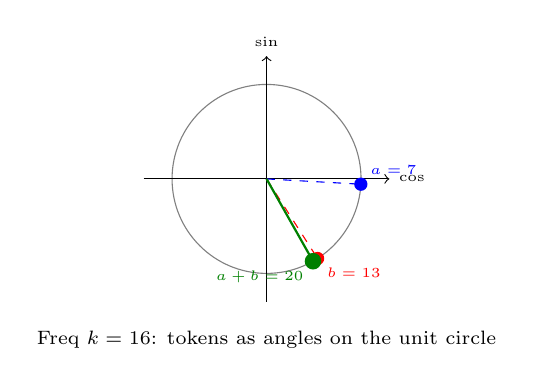
\begin{tikzpicture}[scale=1.2]
    % Unit circle
    \draw[gray, thin] (0,0) circle (1);
    \draw[->] (-1.3,0) -- (1.3,0) node[right] {\tiny $\cos$};
    \draw[->] (0,-1.3) -- (0,1.3) node[above] {\tiny $\sin$};
    \fill[blue] (0.998,-0.056) circle (2pt) node[above right, font=\tiny] {$a=7$};
    \draw[blue, dashed] (0,0) -- (0.998,-0.056);
    \fill[red] (0.540,-0.842) circle (2pt) node[below right, font=\tiny] {$b=13$};
    \draw[red, dashed] (0,0) -- (0.540,-0.842);
    \fill[green!50!black] (0.492,-0.871) circle (2.5pt) node[below left, font=\tiny] {$a+b=20$};
    \draw[green!50!black, thick] (0,0) -- (0.492,-0.871);
    \node[font=\scriptsize] at (0,-1.7) {Freq $k=16$: tokens as angles on the unit circle};
\end{tikzpicture}
\end{center}

\subsubsection{Frequency $k = 31$: $\omega_{31} = \frac{2\pi \cdot 31}{113} = 1.7237$ rad}

\begin{center}
\begin{tabular}{|c|c|c|}
\hline
\textbf{Variable} & \textbf{Meaning} & \textbf{Value} \\ \hline
  $\omega_{31}$ & Angular frequency & $1.7237$ rad \\ \hline
  $n_{\text{neurons}}$ & Neurons assigned to freq $31$ & $0$ \\ \hline
\end{tabular}
\end{center}

\paragraph{Abstract}
Frequency $k = 31$ contributes one cosine wave $\alpha_{31} \cos(\omega_{31}(a+b-c))$ to the logit formula. The embedding encodes tokens as points on a circle of frequency $31$ (i.e., token $t$ maps to angle $\omega_{31} \cdot t$). The MLP's 0 neurons assigned to this frequency collectively compute $\cos(\omega_{31}(a+b))$ and $\sin(\omega_{31}(a+b))$ via the addition formula. The unembedding reads these off via directions $\mathbf{u}_{31}$ and $\mathbf{v}_{31}$ in $W_L$.

\paragraph{Symbolic}
\begin{align}
    \underbrace{W_E[a]}_{\text{row } a \text{ of } W_E} &\xrightarrow{\text{Fourier proj.}} \underbrace{\cos\!\left(\omega_{31} \cdot a\right)}_{\text{cosine at freq } 31},\;\underbrace{\sin\!\left(\omega_{31} \cdot a\right)}_{\text{sine at freq } 31}    \notag \\
    \underbrace{\mathbf{u}_{31}^\top \cdot \text{MLP}(a,b)}_{\text{project MLP onto } \mathbf{u}_{31}} &\approx \underbrace{\alpha_{31}}_{\text{amplitude}} \underbrace{\cos(\omega_{31}(a+b))}_{\text{cosine of sum}}    \notag \\
    \underbrace{\text{Logit contribution}}_{\text{from freq } 31} &= \underbrace{\alpha_{31} \cos(\omega_{31}(a+b-c))}_{\text{peaks at } c = (a+b) \bmod 113}    \notag
\end{align}

\paragraph{Concrete ($a = 7$, $b = 13$)}

\begin{align*}
    \cos(\omega_{31} \cdot 7) &= \cos(1.7237 \times 7) = 0.8774 \\
    \sin(\omega_{31} \cdot 7) &= \sin(1.7237 \times 7) = -0.4798 \\
    \cos(\omega_{31} \cdot 13) &= \cos(1.7237 \times 13) = -0.9143 \\
    \sin(\omega_{31} \cdot 13) &= \sin(1.7237 \times 13) = -0.4050 \\
    \cos(\omega_{31}(7+13)) &= (0.8774)(-0.9143) - (-0.4798)(-0.4050) \\
    &= -0.8022 - 0.1943 = -0.9965 \\
\end{align*}

\begin{center}
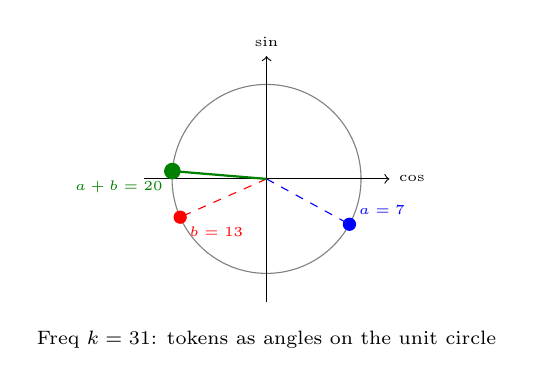
\begin{tikzpicture}[scale=1.2]
    % Unit circle
    \draw[gray, thin] (0,0) circle (1);
    \draw[->] (-1.3,0) -- (1.3,0) node[right] {\tiny $\cos$};
    \draw[->] (0,-1.3) -- (0,1.3) node[above] {\tiny $\sin$};
    \fill[blue] (0.877,-0.480) circle (2pt) node[above right, font=\tiny] {$a=7$};
    \draw[blue, dashed] (0,0) -- (0.877,-0.480);
    \fill[red] (-0.914,-0.405) circle (2pt) node[below right, font=\tiny] {$b=13$};
    \draw[red, dashed] (0,0) -- (-0.914,-0.405);
    \fill[green!50!black] (-0.997,0.083) circle (2.5pt) node[below left, font=\tiny] {$a+b=20$};
    \draw[green!50!black, thick] (0,0) -- (-0.997,0.083);
    \node[font=\scriptsize] at (0,-1.7) {Freq $k=31$: tokens as angles on the unit circle};
\end{tikzpicture}
\end{center}

\subsubsection{Frequency $k = 43$: $\omega_{43} = \frac{2\pi \cdot 43}{113} = 2.3909$ rad}

\begin{center}
\begin{tabular}{|c|c|c|}
\hline
\textbf{Variable} & \textbf{Meaning} & \textbf{Value} \\ \hline
  $\omega_{43}$ & Angular frequency & $2.3909$ rad \\ \hline
  $n_{\text{neurons}}$ & Neurons assigned to freq $43$ & $0$ \\ \hline
\end{tabular}
\end{center}

\paragraph{Abstract}
Frequency $k = 43$ contributes one cosine wave $\alpha_{43} \cos(\omega_{43}(a+b-c))$ to the logit formula. The embedding encodes tokens as points on a circle of frequency $43$ (i.e., token $t$ maps to angle $\omega_{43} \cdot t$). The MLP's 0 neurons assigned to this frequency collectively compute $\cos(\omega_{43}(a+b))$ and $\sin(\omega_{43}(a+b))$ via the addition formula. The unembedding reads these off via directions $\mathbf{u}_{43}$ and $\mathbf{v}_{43}$ in $W_L$.

\paragraph{Symbolic}
\begin{align}
    \underbrace{W_E[a]}_{\text{row } a \text{ of } W_E} &\xrightarrow{\text{Fourier proj.}} \underbrace{\cos\!\left(\omega_{43} \cdot a\right)}_{\text{cosine at freq } 43},\;\underbrace{\sin\!\left(\omega_{43} \cdot a\right)}_{\text{sine at freq } 43}    \notag \\
    \underbrace{\mathbf{u}_{43}^\top \cdot \text{MLP}(a,b)}_{\text{project MLP onto } \mathbf{u}_{43}} &\approx \underbrace{\alpha_{43}}_{\text{amplitude}} \underbrace{\cos(\omega_{43}(a+b))}_{\text{cosine of sum}}    \notag \\
    \underbrace{\text{Logit contribution}}_{\text{from freq } 43} &= \underbrace{\alpha_{43} \cos(\omega_{43}(a+b-c))}_{\text{peaks at } c = (a+b) \bmod 113}    \notag
\end{align}

\paragraph{Concrete ($a = 7$, $b = 13$)}

\begin{align*}
    \cos(\omega_{43} \cdot 7) &= \cos(2.3909 \times 7) = -0.5160 \\
    \sin(\omega_{43} \cdot 7) &= \sin(2.3909 \times 7) = -0.8566 \\
    \cos(\omega_{43} \cdot 13) &= \cos(2.3909 \times 13) = 0.9449 \\
    \sin(\omega_{43} \cdot 13) &= \sin(2.3909 \times 13) = -0.3275 \\
    \cos(\omega_{43}(7+13)) &= (-0.5160)(0.9449) - (-0.8566)(-0.3275) \\
    &= -0.4875 - 0.2805 = -0.7680 \\
\end{align*}

\begin{center}
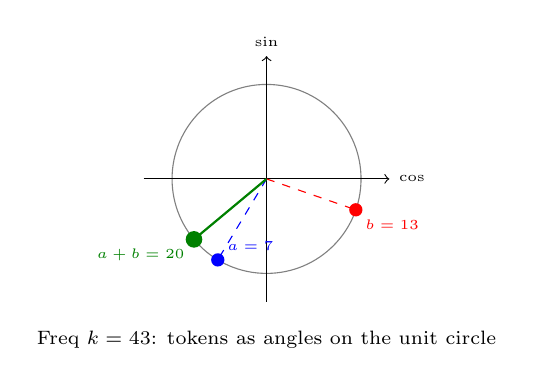
\begin{tikzpicture}[scale=1.2]
    % Unit circle
    \draw[gray, thin] (0,0) circle (1);
    \draw[->] (-1.3,0) -- (1.3,0) node[right] {\tiny $\cos$};
    \draw[->] (0,-1.3) -- (0,1.3) node[above] {\tiny $\sin$};
    \fill[blue] (-0.516,-0.857) circle (2pt) node[above right, font=\tiny] {$a=7$};
    \draw[blue, dashed] (0,0) -- (-0.516,-0.857);
    \fill[red] (0.945,-0.327) circle (2pt) node[below right, font=\tiny] {$b=13$};
    \draw[red, dashed] (0,0) -- (0.945,-0.327);
    \fill[green!50!black] (-0.768,-0.640) circle (2.5pt) node[below left, font=\tiny] {$a+b=20$};
    \draw[green!50!black, thick] (0,0) -- (-0.768,-0.640);
    \node[font=\scriptsize] at (0,-1.7) {Freq $k=43$: tokens as angles on the unit circle};
\end{tikzpicture}
\end{center}

\subsubsection{Frequency $k = 52$: $\omega_{52} = \frac{2\pi \cdot 52}{113} = 2.8914$ rad}

\begin{center}
\begin{tabular}{|c|c|c|}
\hline
\textbf{Variable} & \textbf{Meaning} & \textbf{Value} \\ \hline
  $\omega_{52}$ & Angular frequency & $2.8914$ rad \\ \hline
  $n_{\text{neurons}}$ & Neurons assigned to freq $52$ & $0$ \\ \hline
\end{tabular}
\end{center}

\paragraph{Abstract}
Frequency $k = 52$ contributes one cosine wave $\alpha_{52} \cos(\omega_{52}(a+b-c))$ to the logit formula. The embedding encodes tokens as points on a circle of frequency $52$ (i.e., token $t$ maps to angle $\omega_{52} \cdot t$). The MLP's 0 neurons assigned to this frequency collectively compute $\cos(\omega_{52}(a+b))$ and $\sin(\omega_{52}(a+b))$ via the addition formula. The unembedding reads these off via directions $\mathbf{u}_{52}$ and $\mathbf{v}_{52}$ in $W_L$.

\paragraph{Symbolic}
\begin{align}
    \underbrace{W_E[a]}_{\text{row } a \text{ of } W_E} &\xrightarrow{\text{Fourier proj.}} \underbrace{\cos\!\left(\omega_{52} \cdot a\right)}_{\text{cosine at freq } 52},\;\underbrace{\sin\!\left(\omega_{52} \cdot a\right)}_{\text{sine at freq } 52}    \notag \\
    \underbrace{\mathbf{u}_{52}^\top \cdot \text{MLP}(a,b)}_{\text{project MLP onto } \mathbf{u}_{52}} &\approx \underbrace{\alpha_{52}}_{\text{amplitude}} \underbrace{\cos(\omega_{52}(a+b))}_{\text{cosine of sum}}    \notag \\
    \underbrace{\text{Logit contribution}}_{\text{from freq } 52} &= \underbrace{\alpha_{52} \cos(\omega_{52}(a+b-c))}_{\text{peaks at } c = (a+b) \bmod 113}    \notag
\end{align}

\paragraph{Concrete ($a = 7$, $b = 13$)}

\begin{align*}
    \cos(\omega_{52} \cdot 7) &= \cos(2.8914 \times 7) = 0.1797 \\
    \sin(\omega_{52} \cdot 7) &= \sin(2.8914 \times 7) = 0.9837 \\
    \cos(\omega_{52} \cdot 13) &= \cos(2.8914 \times 13) = 0.9938 \\
    \sin(\omega_{52} \cdot 13) &= \sin(2.8914 \times 13) = -0.1110 \\
    \cos(\omega_{52}(7+13)) &= (0.1797)(0.9938) - (0.9837)(-0.1110) \\
    &= 0.1786 - -0.1092 = 0.2878 \\
\end{align*}

\begin{center}
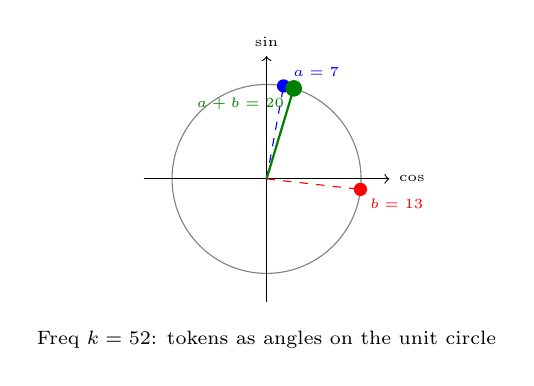
\begin{tikzpicture}[scale=1.2]
    % Unit circle
    \draw[gray, thin] (0,0) circle (1);
    \draw[->] (-1.3,0) -- (1.3,0) node[right] {\tiny $\cos$};
    \draw[->] (0,-1.3) -- (0,1.3) node[above] {\tiny $\sin$};
    \fill[blue] (0.180,0.984) circle (2pt) node[above right, font=\tiny] {$a=7$};
    \draw[blue, dashed] (0,0) -- (0.180,0.984);
    \fill[red] (0.994,-0.111) circle (2pt) node[below right, font=\tiny] {$b=13$};
    \draw[red, dashed] (0,0) -- (0.994,-0.111);
    \fill[green!50!black] (0.288,0.958) circle (2.5pt) node[below left, font=\tiny] {$a+b=20$};
    \draw[green!50!black, thick] (0,0) -- (0.288,0.958);
    \node[font=\scriptsize] at (0,-1.7) {Freq $k=52$: tokens as angles on the unit circle};
\end{tikzpicture}
\end{center}

\subsubsection{Frequency $k = 53$: $\omega_{53} = \frac{2\pi \cdot 53}{113} = 2.9470$ rad}

\begin{center}
\begin{tabular}{|c|c|c|}
\hline
\textbf{Variable} & \textbf{Meaning} & \textbf{Value} \\ \hline
  $\omega_{53}$ & Angular frequency & $2.9470$ rad \\ \hline
  $n_{\text{neurons}}$ & Neurons assigned to freq $53$ & $0$ \\ \hline
\end{tabular}
\end{center}

\paragraph{Abstract}
Frequency $k = 53$ contributes one cosine wave $\alpha_{53} \cos(\omega_{53}(a+b-c))$ to the logit formula. The embedding encodes tokens as points on a circle of frequency $53$ (i.e., token $t$ maps to angle $\omega_{53} \cdot t$). The MLP's 0 neurons assigned to this frequency collectively compute $\cos(\omega_{53}(a+b))$ and $\sin(\omega_{53}(a+b))$ via the addition formula. The unembedding reads these off via directions $\mathbf{u}_{53}$ and $\mathbf{v}_{53}$ in $W_L$.

\paragraph{Symbolic}
\begin{align}
    \underbrace{W_E[a]}_{\text{row } a \text{ of } W_E} &\xrightarrow{\text{Fourier proj.}} \underbrace{\cos\!\left(\omega_{53} \cdot a\right)}_{\text{cosine at freq } 53},\;\underbrace{\sin\!\left(\omega_{53} \cdot a\right)}_{\text{sine at freq } 53}    \notag \\
    \underbrace{\mathbf{u}_{53}^\top \cdot \text{MLP}(a,b)}_{\text{project MLP onto } \mathbf{u}_{53}} &\approx \underbrace{\alpha_{53}}_{\text{amplitude}} \underbrace{\cos(\omega_{53}(a+b))}_{\text{cosine of sum}}    \notag \\
    \underbrace{\text{Logit contribution}}_{\text{from freq } 53} &= \underbrace{\alpha_{53} \cos(\omega_{53}(a+b-c))}_{\text{peaks at } c = (a+b) \bmod 113}    \notag
\end{align}

\paragraph{Concrete ($a = 7$, $b = 13$)}

\begin{align*}
    \cos(\omega_{53} \cdot 7) &= \cos(2.9470 \times 7) = -0.2070 \\
    \sin(\omega_{53} \cdot 7) &= \sin(2.9470 \times 7) = 0.9783 \\
    \cos(\omega_{53} \cdot 13) &= \cos(2.9470 \times 13) = 0.8187 \\
    \sin(\omega_{53} \cdot 13) &= \sin(2.9470 \times 13) = 0.5742 \\
    \cos(\omega_{53}(7+13)) &= (-0.2070)(0.8187) - (0.9783)(0.5742) \\
    &= -0.1695 - 0.5618 = -0.7312 \\
\end{align*}

\begin{center}
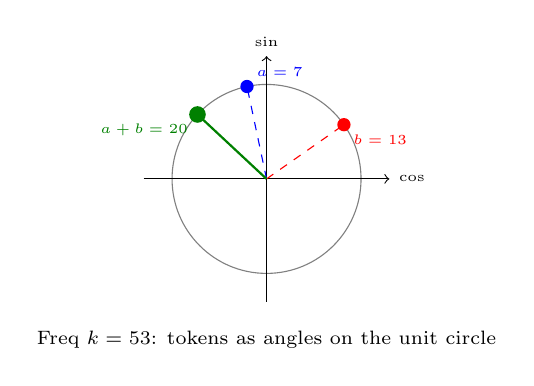
\begin{tikzpicture}[scale=1.2]
    % Unit circle
    \draw[gray, thin] (0,0) circle (1);
    \draw[->] (-1.3,0) -- (1.3,0) node[right] {\tiny $\cos$};
    \draw[->] (0,-1.3) -- (0,1.3) node[above] {\tiny $\sin$};
    \fill[blue] (-0.207,0.978) circle (2pt) node[above right, font=\tiny] {$a=7$};
    \draw[blue, dashed] (0,0) -- (-0.207,0.978);
    \fill[red] (0.819,0.574) circle (2pt) node[below right, font=\tiny] {$b=13$};
    \draw[red, dashed] (0,0) -- (0.819,0.574);
    \fill[green!50!black] (-0.731,0.682) circle (2.5pt) node[below left, font=\tiny] {$a+b=20$};
    \draw[green!50!black, thick] (0,0) -- (-0.731,0.682);
    \node[font=\scriptsize] at (0,-1.7) {Freq $k=53$: tokens as angles on the unit circle};
\end{tikzpicture}
\end{center}

\end{document}
